% !TEX TS-program = xelatex

\documentclass[a4paper,12pt]{extarticle}
% !TEX TS-program = xelatex

% Document class and spacing
\renewcommand{\baselinestretch}{1.4}

% Packages
\usepackage{graphicx}
\usepackage{amsmath, amssymb}
\usepackage{geometry}
\usepackage{setspace}
\usepackage{fancyhdr}
\usepackage{titlesec}
\usepackage[colorlinks=true, linkcolor=darkblue, urlcolor=darkblue, citecolor=darkblue]{hyperref}
\usepackage[dvipsnames]{xcolor}
\usepackage{tcolorbox}
\usepackage{calc}
\usepackage{eso-pic}
\usepackage{fontspec}
\usepackage{natbib}
\usepackage{float}
\usepackage{caption}

\bibliographystyle{plain}

% English Fonts - Times New Roman
\setmainfont{Times New Roman}

% Colors
\definecolor{darkblue}{rgb}{.204,.353,.541}
\definecolor{lightblue}{RGB}{210, 227, 245}

% Section box command
\newcommand{\sectionbox}[1]{%
  \begin{tcolorbox}[colback=lightblue, colframe=lightblue, width=\linewidth, sharp corners]
    \color{darkblue} \eighteenpt \bfseries #1
  \end{tcolorbox}
}

% Section and subsection formatting
\titleformat{\section}
{\eighteenpt\bfseries}{} {0em} {\sectionbox}
\titlespacing{\section}{0pt}{12pt}{6pt}

\titleformat{\subsection}
{\color{darkblue}\sixteenpt\bfseries}
{\thesubsection}{1em}
{}

% Font size commands
\newcommand{\sixteenpt}{\fontsize{16pt}{18pt}\selectfont}
\newcommand{\eighteenpt}{\fontsize{18pt}{20pt}\selectfont}
\newcommand{\twentytwopt}{\fontsize{22pt}{24pt}\selectfont}
\newcommand{\twentyeightpt}{\fontsize{28pt}{30pt}\selectfont}

% Custom title page
\makeatletter
\def\maketitle{
  \begin{center}
    \begin{tabular}{ p{3cm} p{7cm} p{3.5cm} }
      
\includegraphics[width=3cm]{assets/images/logo.png} &
      \vspace{-3cm}
      \begin{center}
        {\sixteenpt{\textbf{University of Tehran}}\\[0.2cm]
          \sixteenpt{\textbf{College of Engineering}}\\[0.2cm]
        \sixteenpt{\textbf{Department of Electrical and Computer Engineering}}}
      \end{center}
      &
      
\includegraphics[width=3.5cm]{assets/images/eng-logo.png} 
    \end{tabular}

    \vspace{4cm}
    {\twentyeightpt \textbf{\CourseName}} \\
    \vspace{0.5cm}
    {\twentytwopt \textbf{\@title}} \\
    \vspace{2cm}
    {\eighteenpt \textbf{Instructors: Dr. Bahrak, Dr. Yaghoobzadeh}} \\
    \vspace{2cm}
    {\sixteenpt \textbf{Prepared by:}} \\
    \vspace{0.5cm}
    {\eighteenpt \textbf{\@author}} \\
    {\eighteenpt \textbf{Student No: \SNum}} \\
    \vfill
    {\sixteenpt \@date}
  \end{center}
}
\makeatother

\geometry{a4paper, margin=1in}
\graphicspath{{assets/images/}}

% Document Info
\newcommand{\CourseName}{Introduction to Data Science}
\newcommand{\assignNum}{3}
\title{Assignment \assignNum}

% Group Members Configuration
\author{
  \begin{tabular}{c}
  Parsa Saeednia (810102460) \\
  Mohammad Hossein Mazaheri (810102585) \\
  Mohammad Reza Pirhadi (810102423)
  \end{tabular}
}
\date{\today}

\makeatletter
\def\maketitle{
  \begin{center}
    \begin{tabular}{ p{3cm} p{7cm} p{3.5cm} }
      
\includegraphics[width=3cm]{logo.png} &
      \vspace{-3cm}
      \begin{center}
        {\sixteenpt{\textbf{University of Tehran}}\\[0.2cm]
        \sixteenpt{\textbf{College of Engineering}}\\[0.2cm]
        \sixteenpt{\textbf{Department of Electrical and Computer Engineering}}}
      \end{center}
      &
      
\includegraphics[width=3.5cm]{eng-logo.png} 
    \end{tabular}

    \vspace{4cm}
    {\twentyeightpt \textbf{\CourseName}} \\
    \vspace{0.5cm}
    {\twentytwopt \textbf{\@title}} \\
    \vspace{2cm}
    {\sixteenpt \@author} \\
    \vspace{2cm}
    {\sixteenpt \@date}
  \end{center}
  \thispagestyle{empty}
  \clearpage
}
\makeatother

\begin{document}

\maketitle

\tableofcontents
\clearpage

\begin{abstract}
This report outlines the methodology, implementation, and evaluation of our approaches for Assignment 3. The project is divided into multiple distinct tasks, ranging from data exploration to advanced predictive modeling. In Task 3, we specifically address a complex Information Retrieval problem, transitioning from standard tabular classification to a Learning to Rank (LTR) pipeline to effectively match candidates to job postings under extreme class imbalance.
\end{abstract}

\clearpage

% ==========================================
% TASK 1
% ==========================================
\section{Task 1: [Insert Task 1 Title]}

\subsection{Exploratory Data Analysis}
% Insert Task 1 EDA details here

\subsection{Preprocessing}
% Insert Task 1 Preprocessing details here

\subsection{Modeling \& Evaluation}
% Insert Task 1 Modeling details here

\clearpage

% ==========================================
% TASK 2
% ==========================================
\section{Task 2: [Insert Task 2 Title]}

\subsection{Exploratory Data Analysis}
% Insert Task 2 EDA details here

\subsection{Preprocessing}
% Insert Task 2 Preprocessing details here

\subsection{Modeling \& Evaluation}
% Insert Task 2 Modeling details here

\clearpage

% ==========================================
% TASK 3
% ==========================================
\section{Task 3: Candidate Ranking (Learning to Rank)}

\subsection{Introduction}
Task 3 requires evaluating and ordering job candidates based on their qualifications. Because the objective is to rank candidates for specific job postings rather than predict a global probability, we approached this as an Information Retrieval problem utilizing a \textbf{Learning to Rank} methodology. 

\subsection{Exploratory Data Analysis (EDA)}
Extensive data exploration was required to understand the underlying structure of the applications and guide our feature engineering.

\subsubsection{Target Variable Imbalance}
Our initial analysis revealed a severe class imbalance. As shown in Figure \ref{fig:target_distribution}, the vast majority of applications are labeled 0 (Poor Fit), with true ideal candidates (Label 4) being extremely rare. Consequently, standard classification accuracy is mathematically flawed for this task, necessitating the use of ranking-specific metrics like NDCG.

\begin{figure}[H]
    \centering
    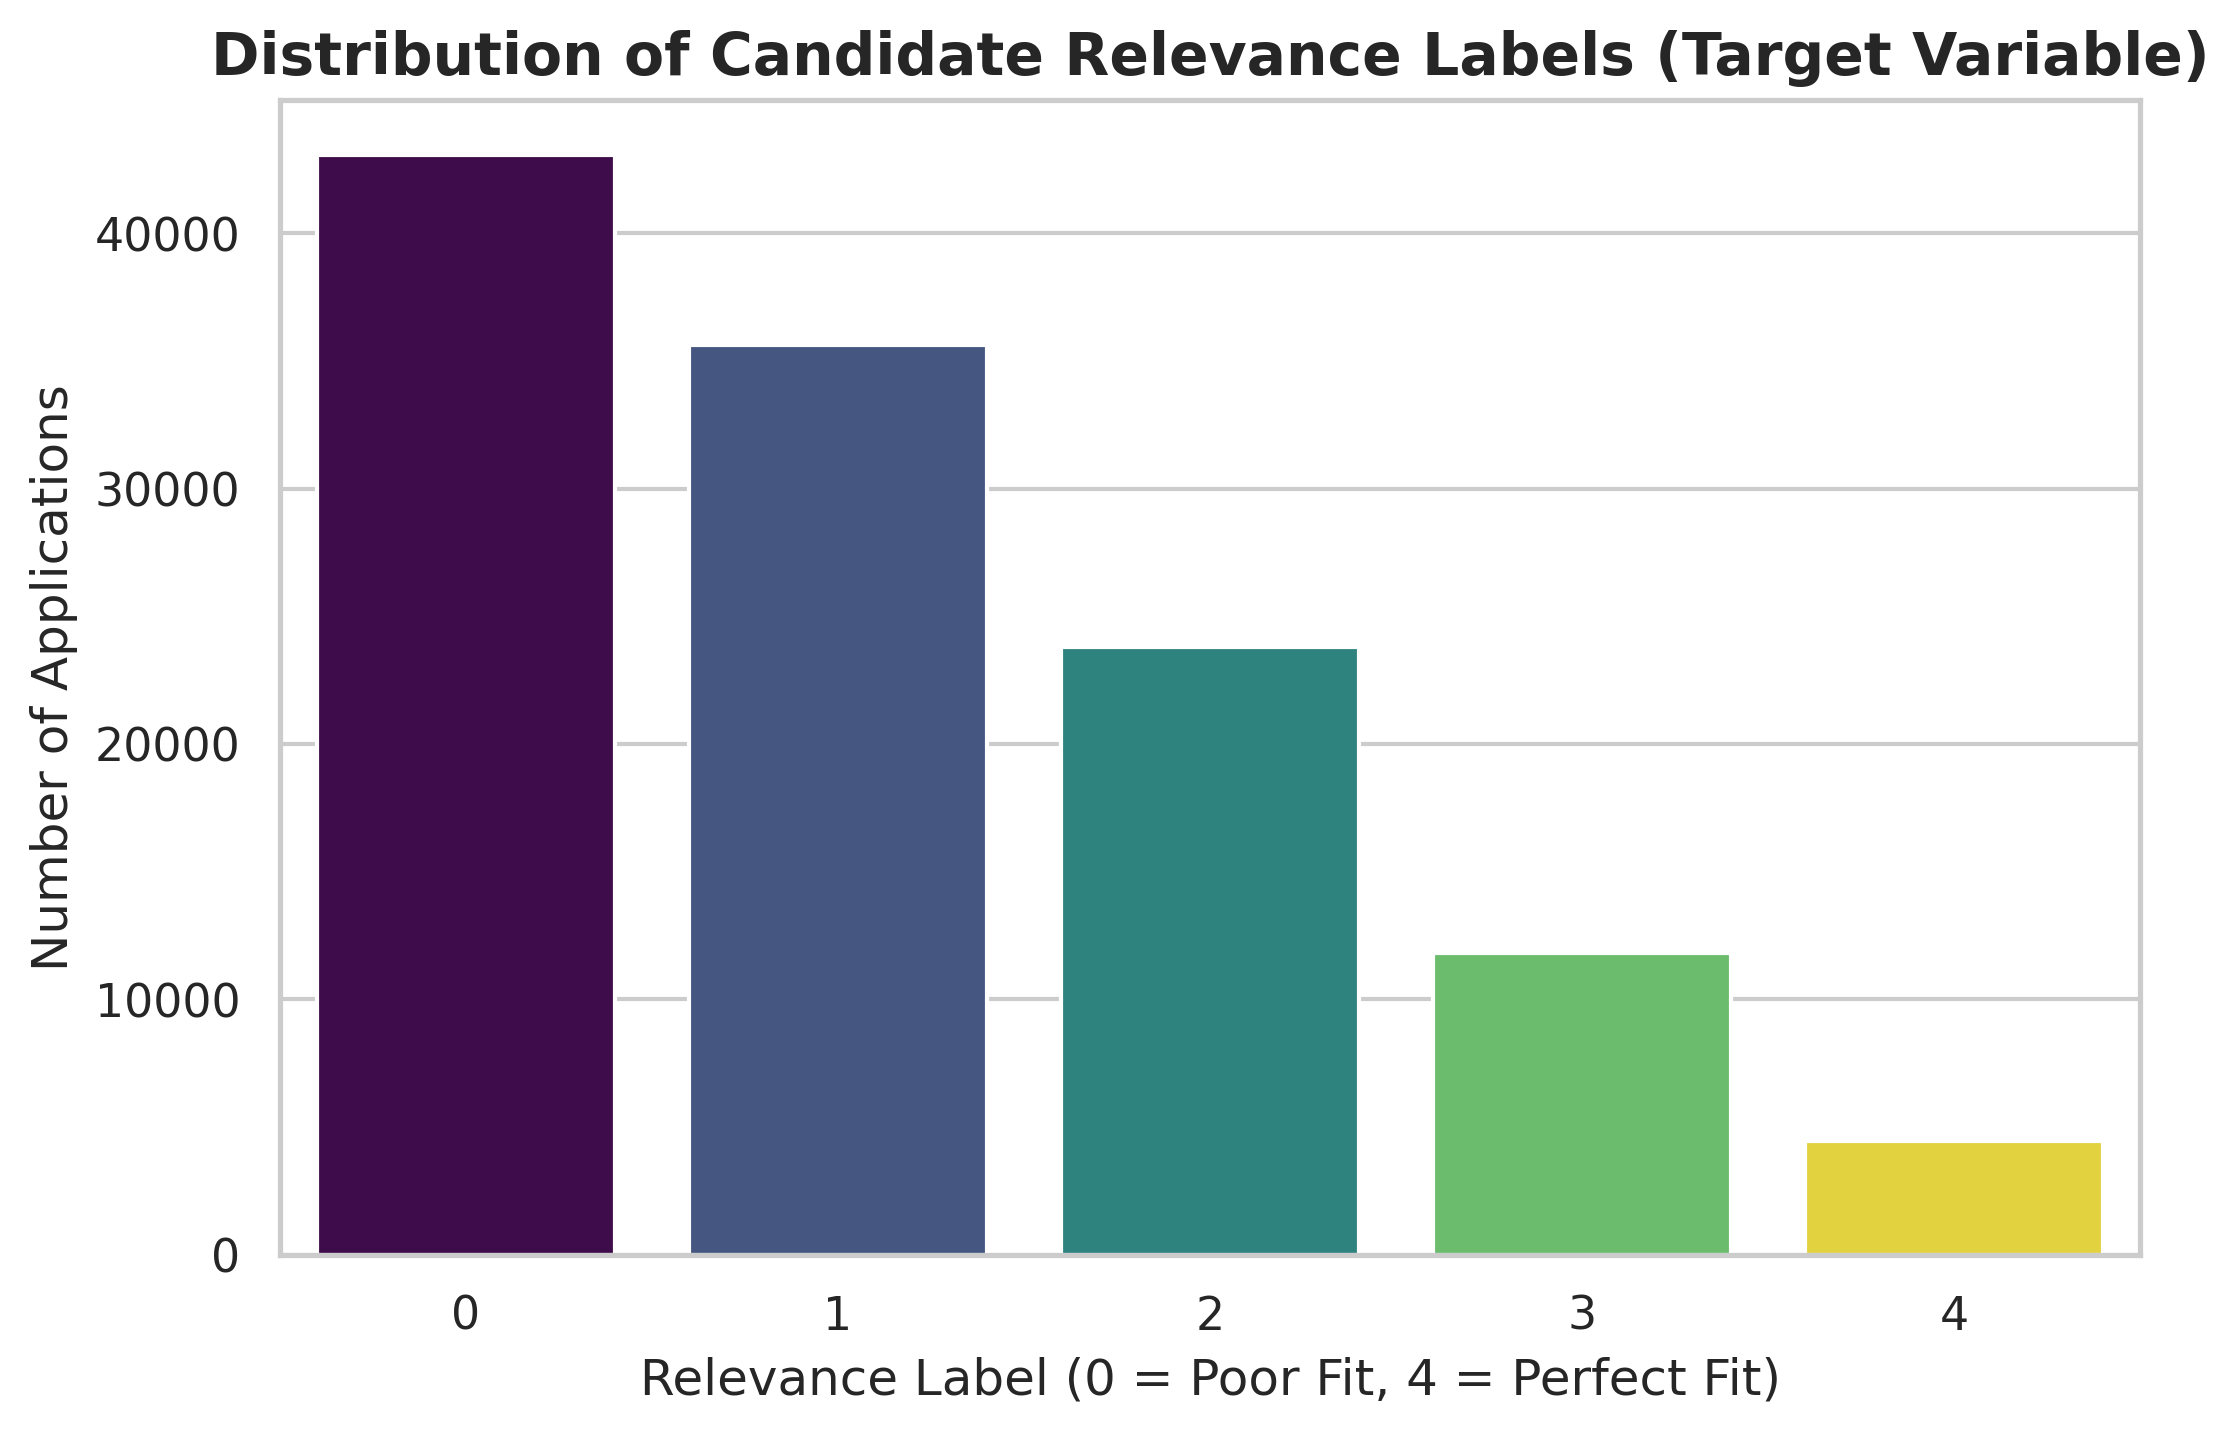
\includegraphics[width=0.8\textwidth]{01_target_distribution.png}
    \caption{Distribution of candidate relevance labels showcasing extreme class imbalance.}
    \label{fig:target_distribution}
\end{figure}

\subsubsection{The Currency Discrepancy}
While analyzing salary features, we discovered a massive scaling mismatch. The job board's maximum salary distributions contained extreme outliers in the billions, while candidate expectations remained in a tight, lower distribution (Figure \ref{fig:currency}). This visual confirmation proved that \texttt{salary\_max} was listed in un-normalized local currencies (e.g., IRR), while candidate expectations (\texttt{expected\_salary}) were already globally normalized to USD.

\begin{figure}[H]
    \centering
    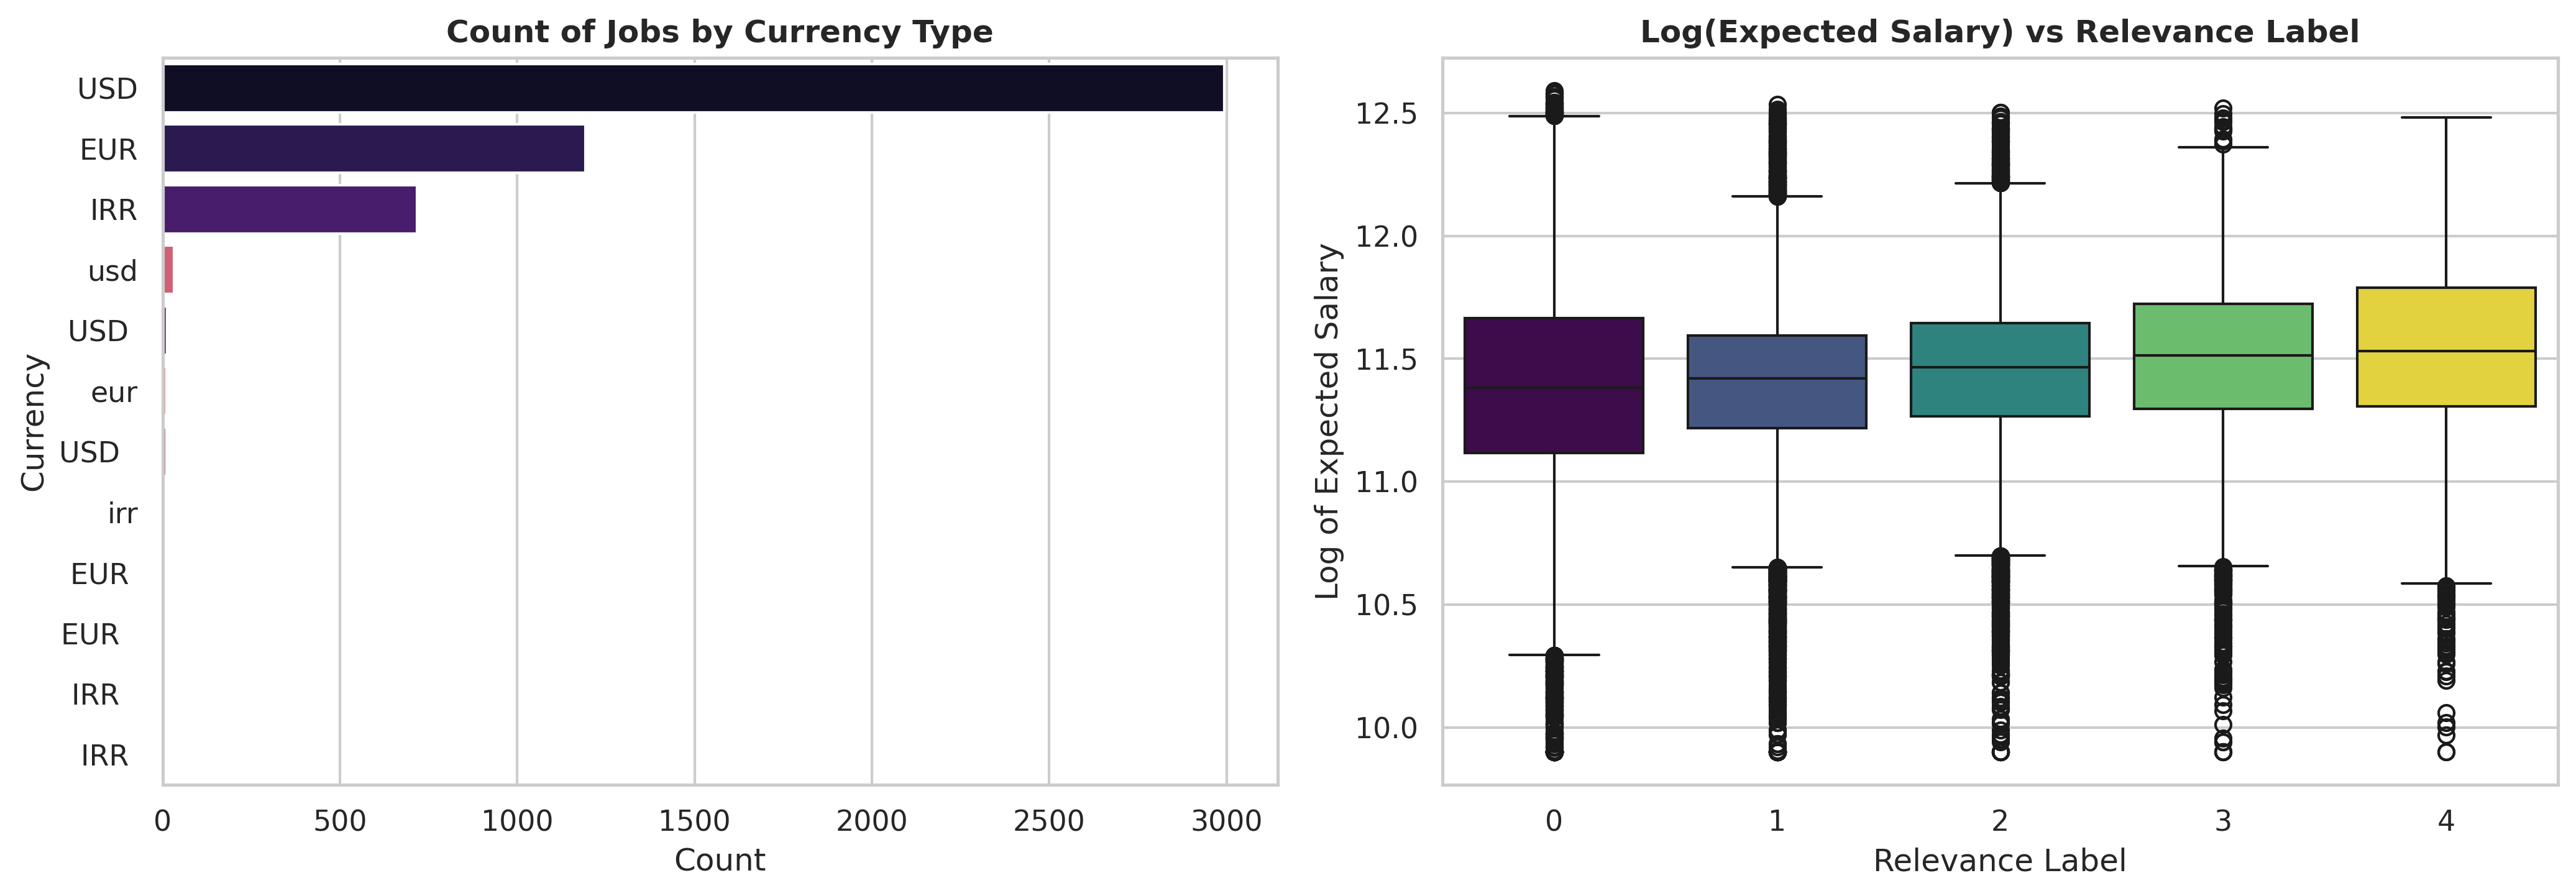
\includegraphics[width=0.9\textwidth]{02_currency_and_salary.png}
    \caption{Salary distribution anomalies highlighting the need for dynamic currency unification.}
    \label{fig:currency}
\end{figure}

\subsubsection{Temporal Distributions \& Interaction Proxies}
We mapped the temporal distribution of applications to establish a safe cutoff date for our validation set, preventing future data leakage (Figure \ref{fig:temporal}). Furthermore, early boxplots (Figure \ref{fig:exp_gap}) suggested that engineering an "Experience Gap" feature (candidate experience minus minimum job experience) yielded a much higher signal-to-noise ratio than raw experience alone.

\begin{figure}[H]
    \centering
    \begin{minipage}{0.48\textwidth}
        \centering
        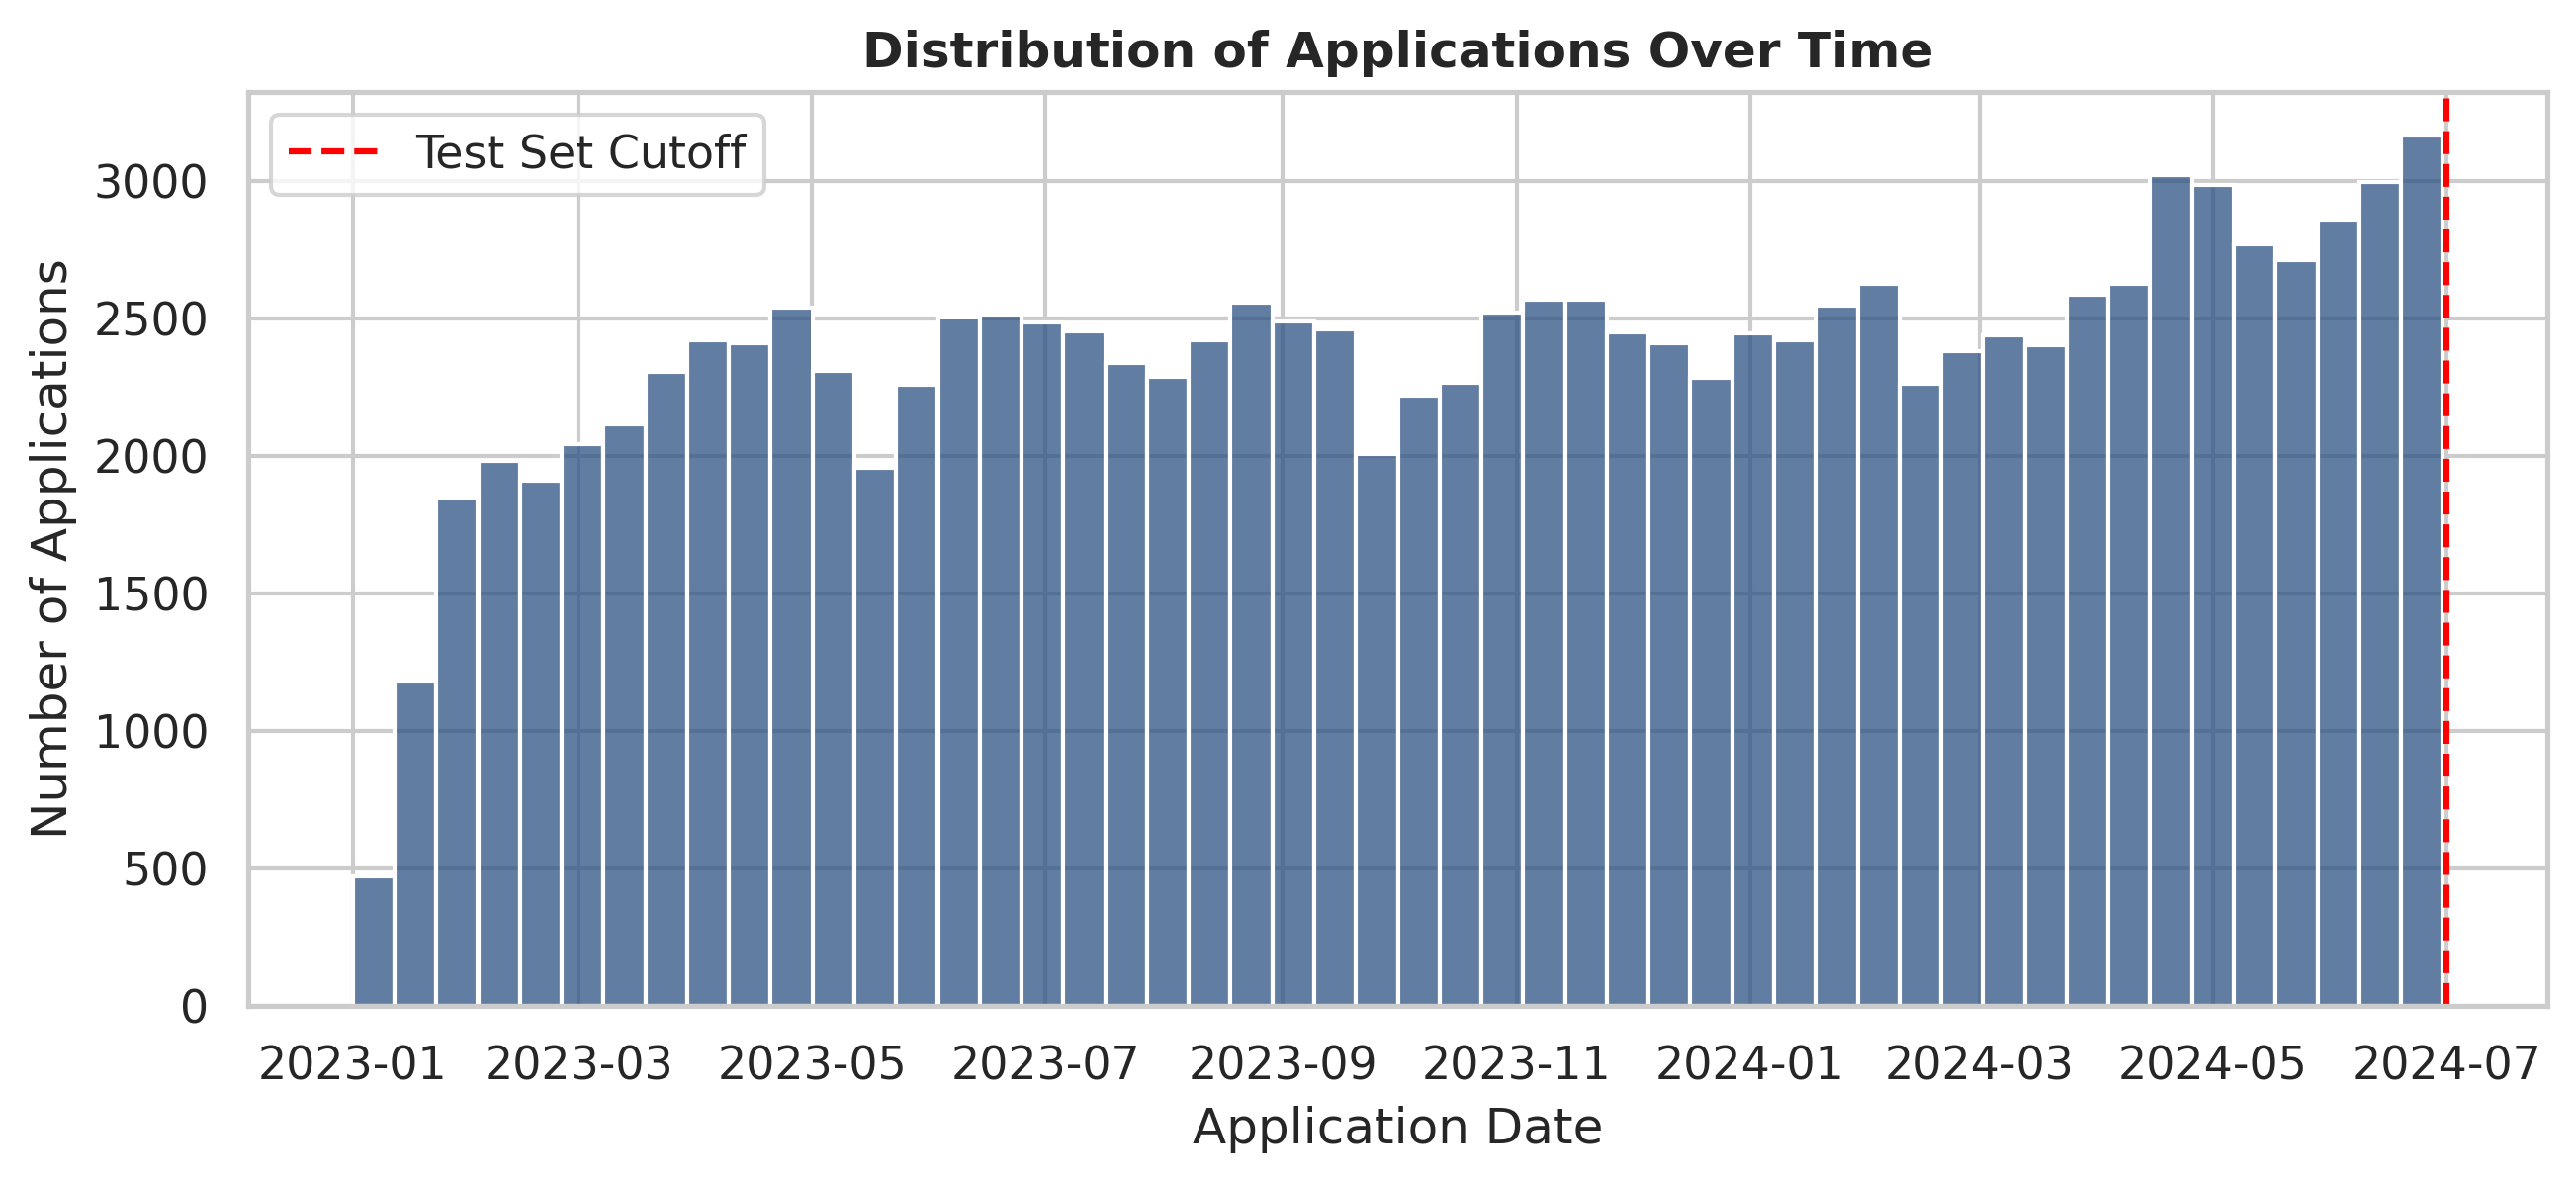
\includegraphics[width=\linewidth]{03_temporal_distribution.png}
        \caption{Timeline of applications used to design the temporal validation split.}
        \label{fig:temporal}
    \end{minipage}\hfill
    \begin{minipage}{0.48\textwidth}
        \centering
        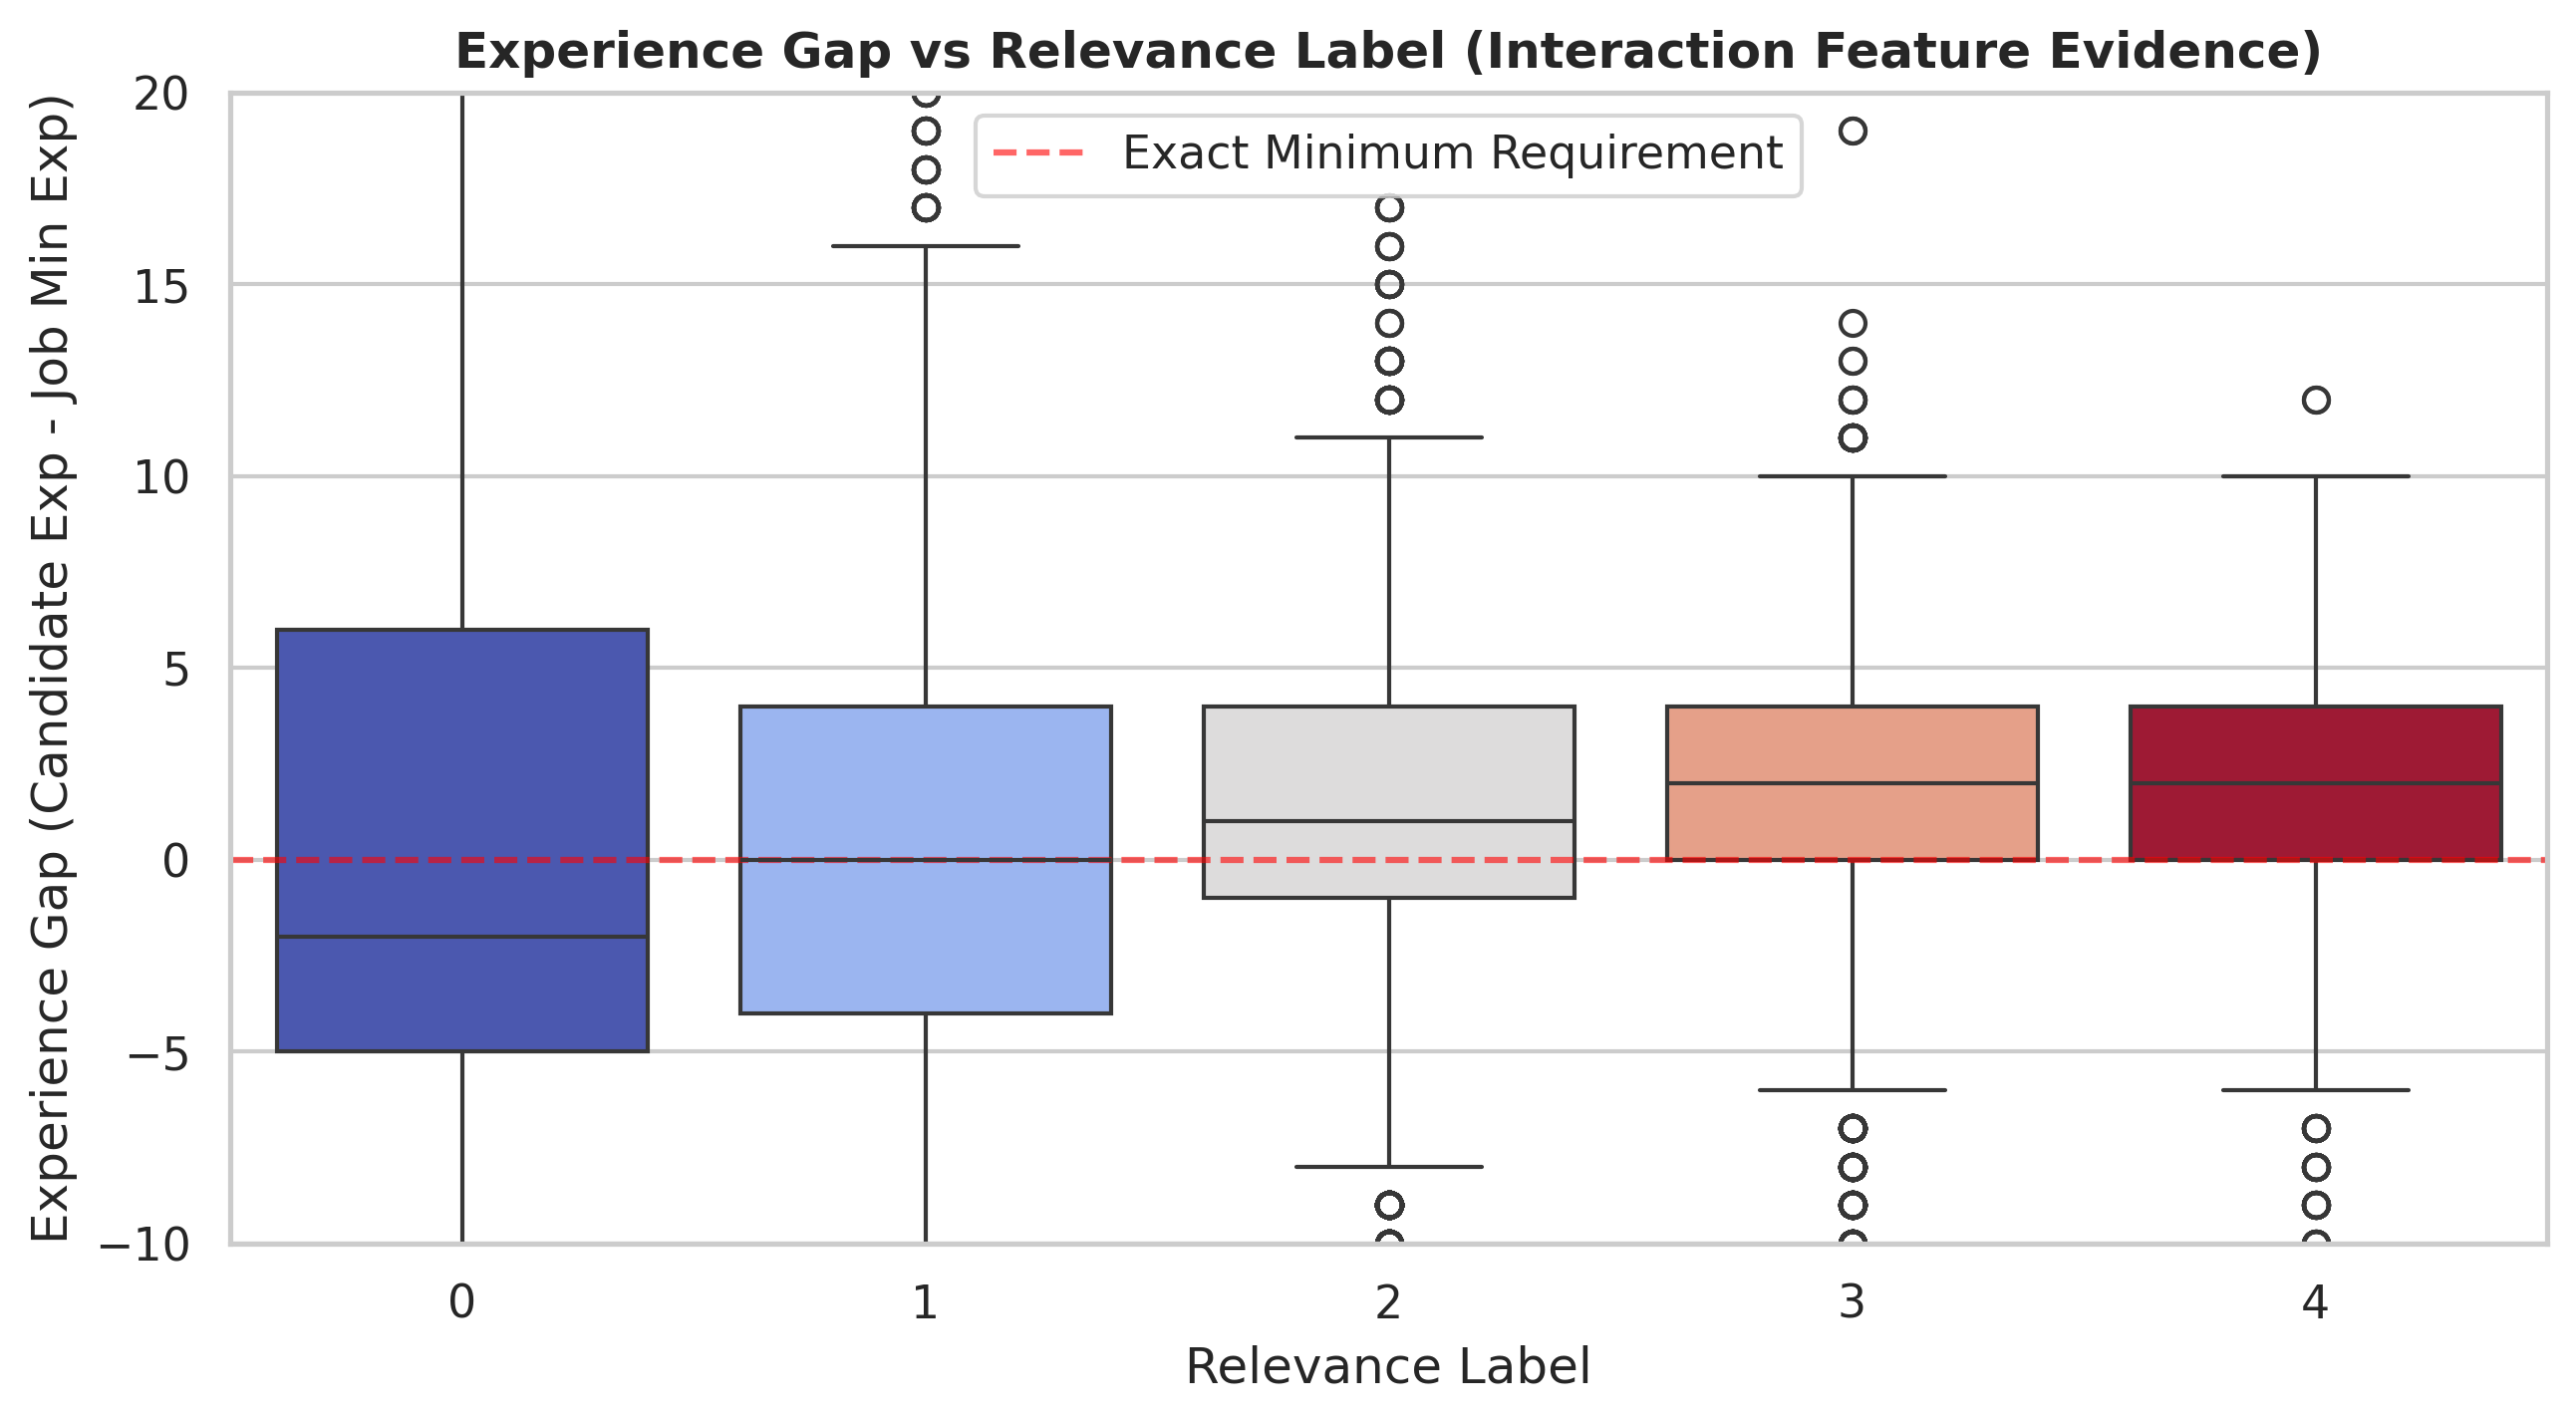
\includegraphics[width=\linewidth]{04_experience_gap_proxy.png}
        \caption{Experience Gap proxy highlighting correlation with relevance.}
        \label{fig:exp_gap}
    \end{minipage}
\end{figure}

\subsection{Preprocessing \& Data Integration}
To prepare the dataset for the ranking algorithm, we merged the relational tables and resolved the identified data integrity issues:
\begin{itemize}
    \item \textbf{Text Standardization:} Categorical columns exhibited severe casing and whitespace inconsistencies. A global normalization function was applied to lowercase and strip all strings to prevent fragmented category encoding.
    \item \textbf{Currency Unification:} Based on our EDA findings, we implemented a parameterized normalizer that applied a historical exchange rate (IRR to USD) strictly to the job postings, establishing a unified USD mathematical baseline for feature comparisons.
\end{itemize}

\subsection{Interaction Feature Engineering}
A ranking model relies heavily on the interaction between the query (the job) and the document (the candidate). We dropped non-predictive categorical strings and engineered 19 direct features (17 interactions and 2 target encodings). The final model utilized 29 total features, heavily prioritizing these newly created relationships:
\begin{enumerate}
    \item \textbf{Skill Metrics:} We calculated the Jaccard Similarity between skillsets (\texttt{skill\_overlap\_score}), alongside raw string-split counts for both candidates and jobs (\texttt{cand\_skill\_count}, \texttt{job\_skill\_count}) and their relative fraction (\texttt{skill\_count\_ratio}).
    \item \textbf{Experience \& Seniority:} We extracted continuous experience differences (\texttt{experience\_gap}), mapped title keywords (e.g., "Senior", "Junior") to ordinal values (\texttt{cand\_seniority}, \texttt{job\_seniority}), and checked for strict alignment (\texttt{seniority\_match}).
    \item \textbf{Salary \& Budget:} We formulated a boolean budget check (\texttt{salary\_within\_budget}) and a continuous float representing the ratio of candidate expectations to the maximum budget (\texttt{salary\_ratio}).
    \item \textbf{Categorical Ordinals \& Matches:} Textual classifications were converted into clean numeric scales for \texttt{education\_score}, \texttt{english\_score}, and \texttt{company\_size\_num}, while geographic compatibility was flagged via \texttt{location\_match}.
    \item \textbf{Temporal \& Effort Filters:} We extracted the number of candidate certifications (\texttt{cert\_count}) and computed the age of the job posting (\texttt{job\_age\_days}) alongside the age of the candidate's account (\texttt{acc\_age\_days}) at the time of application to penalize low-effort or automated mass-applying behavior.
\end{enumerate}

\subsubsection{Double Out-of-Fold (OOF) Target Encoding}
The candidate's \texttt{current\_title} and \texttt{university} contained massive predictive power (prestige and specific role relevance) but possessed high cardinality, risking data leakage and dimensionality explosion. We implemented a Group K-Fold Out-of-Fold Target Encoder with a mathematical smoothing parameter. By encoding these two strings using the target averages of out-of-fold applications (grouped safely by \texttt{job\_id}), we safely provided the model with these critical signals.

\subsection{Model Development \& Hyperparameter Tuning}
We utilized \texttt{LightGBM Ranker} with the \texttt{lambdarank} objective function. To simulate the hidden test environment, we split the training data using an application cutoff date of \texttt{2024-05-01}. The matrices were explicitly sorted and grouped by \texttt{job\_id}.

A dynamic tuning loop found that a learning rate of 0.05 combined with a 5-fold OOF smoothing factor provided the highest stability. As shown in Figure \ref{fig:feature_importance}, our engineered interaction features—specifically the continuous skill overlaps, experience gaps, and OOF encoded titles—completely dominated the model's decision-making process.

\begin{figure}[H]
    \centering
    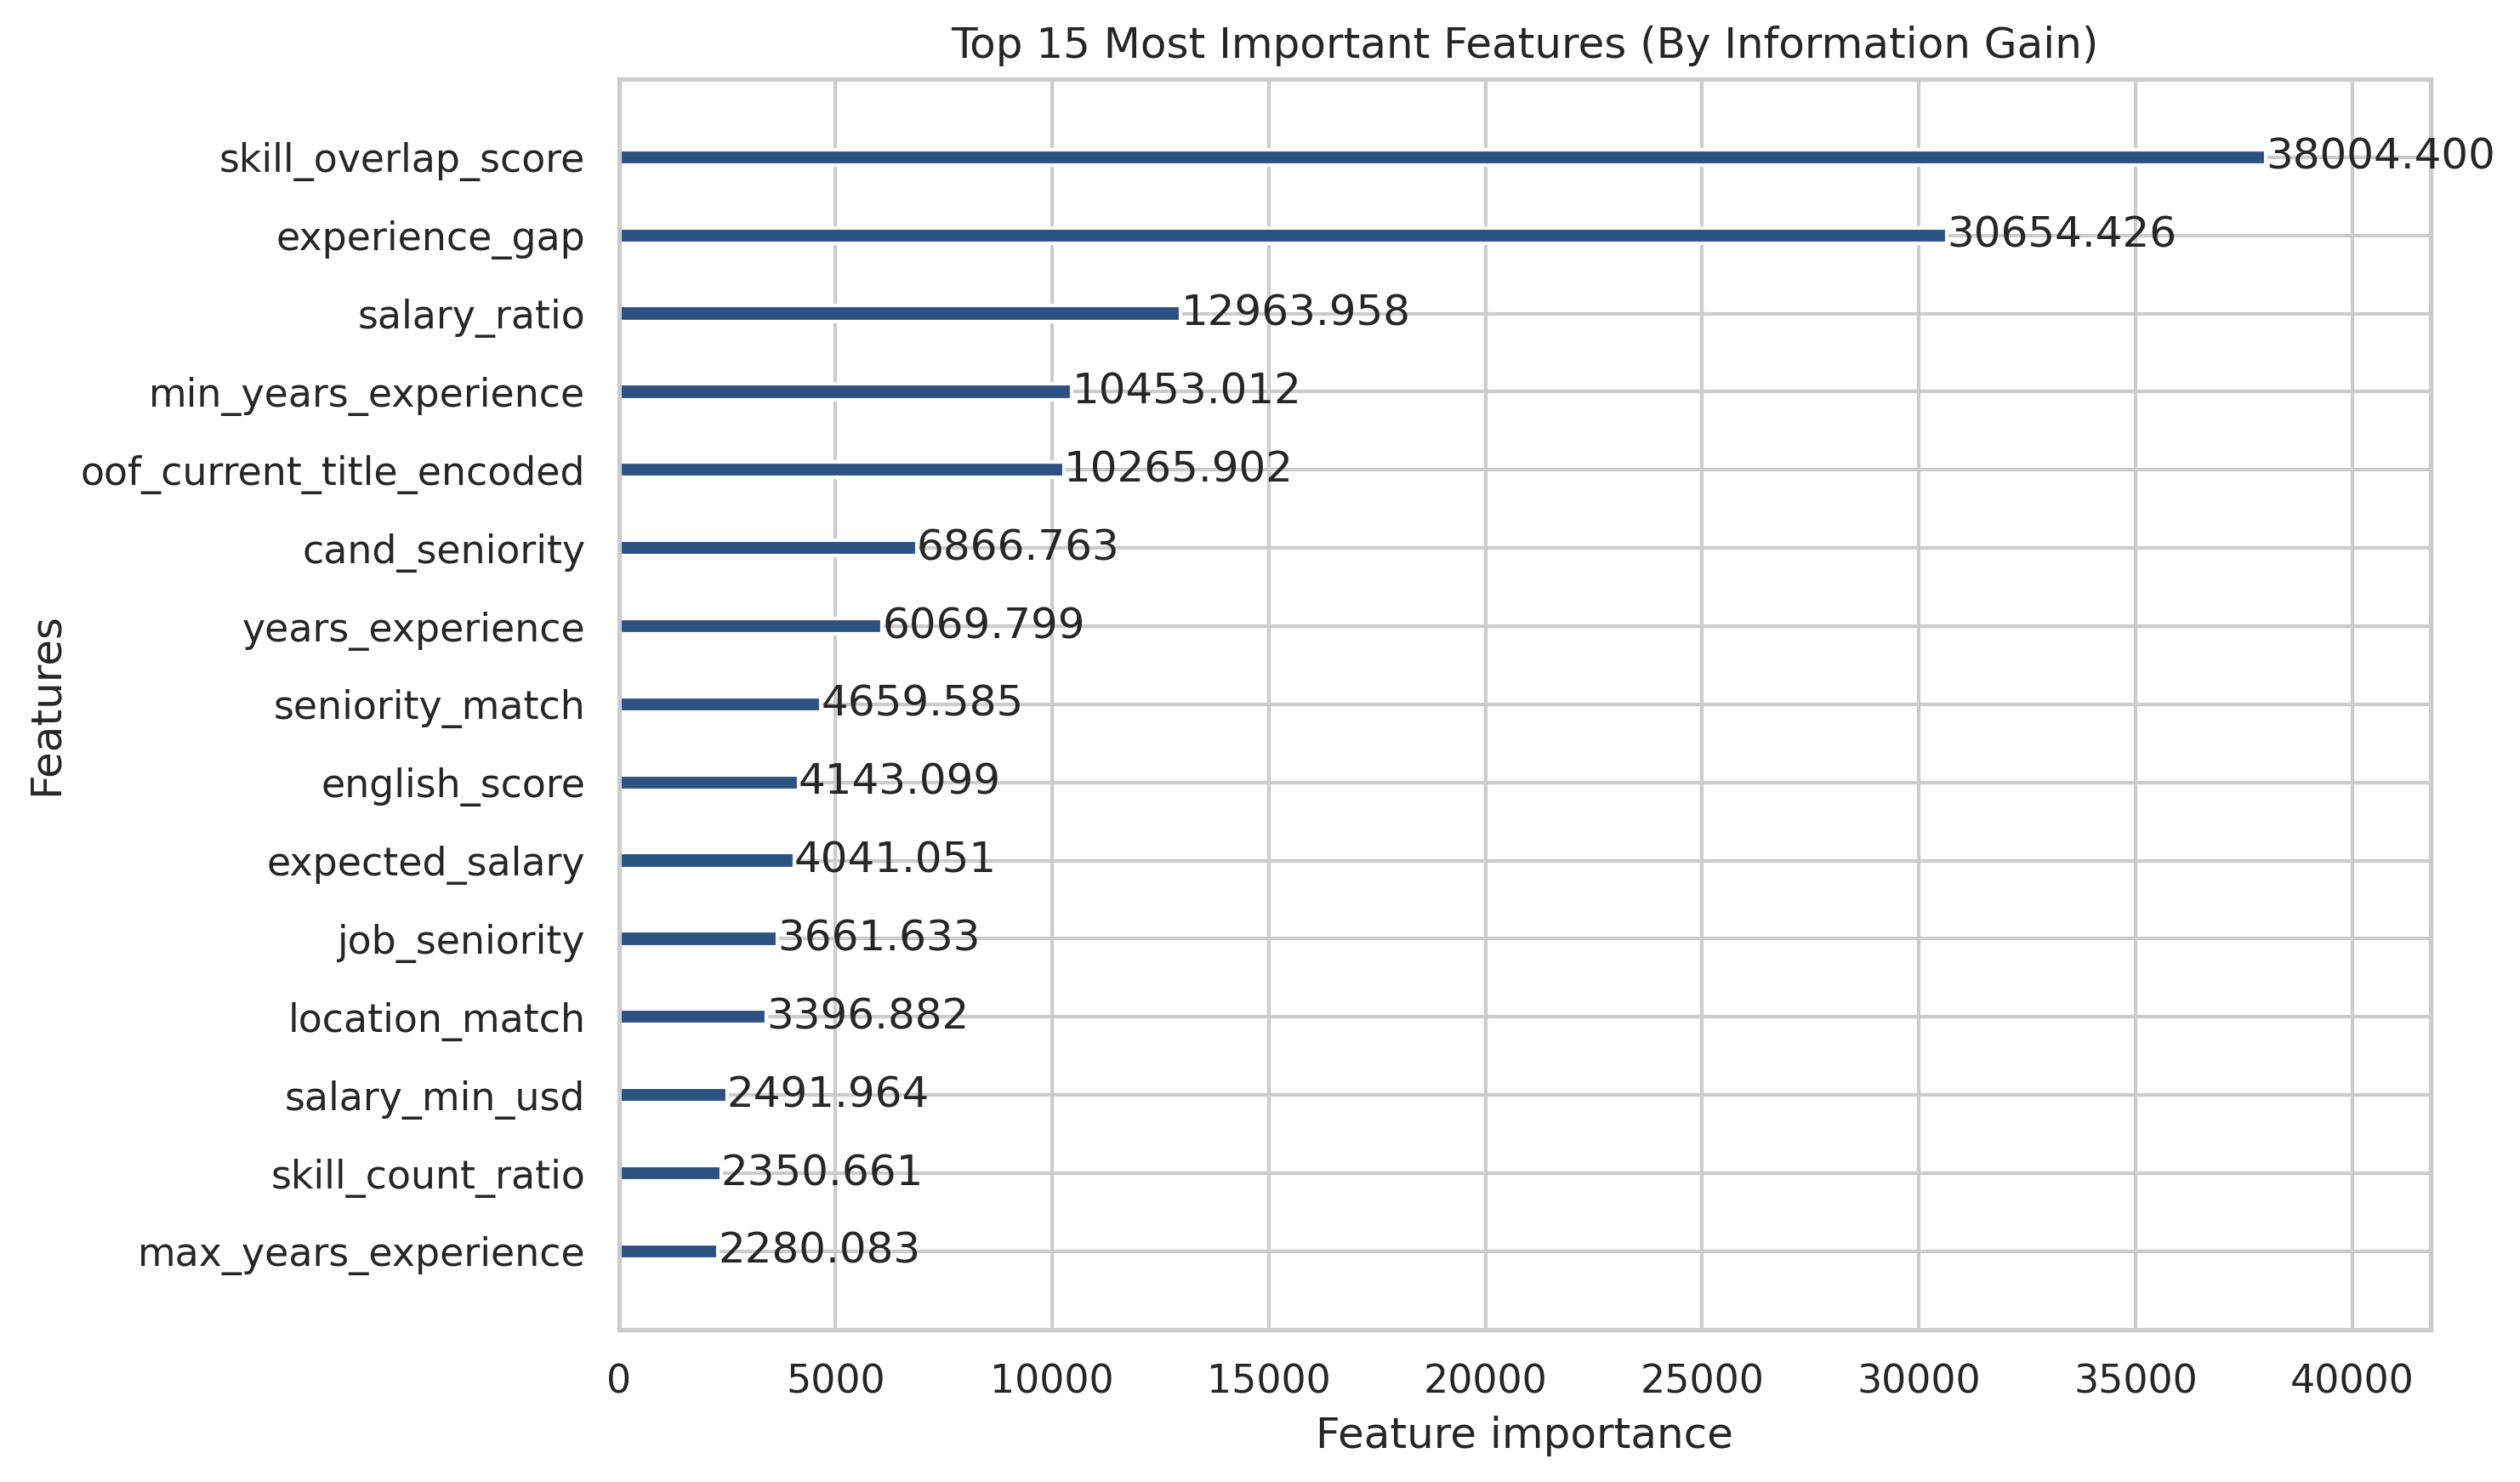
\includegraphics[width=0.9\textwidth]{05_feature_importance.png}
    \caption{Top 15 Most Important Features (By Information Gain). Engineered interaction features drastically outperformed raw dataset variables.}
    \label{fig:feature_importance}
\end{figure}

\subsection{Comprehensive Evaluation}
Because standard libraries often abstract Information Retrieval metrics, we implemented custom Python evaluations for \textbf{NDCG@10} (Normalized Discounted Cumulative Gain) and \textbf{MAP@5} (Mean Average Precision). 

The baseline validation model achieved an excellent custom \textbf{Mean NDCG@10 of $\sim$0.901} and a \textbf{MAP@5 of $\sim$0.731} (Figure \ref{fig:evaluation_dist}). This confirms the model successfully pulls rare, highly-qualified applicants out of the severe class imbalance and positions them within the top recommendations for recruiters. 

\begin{figure}[H]
    \centering
    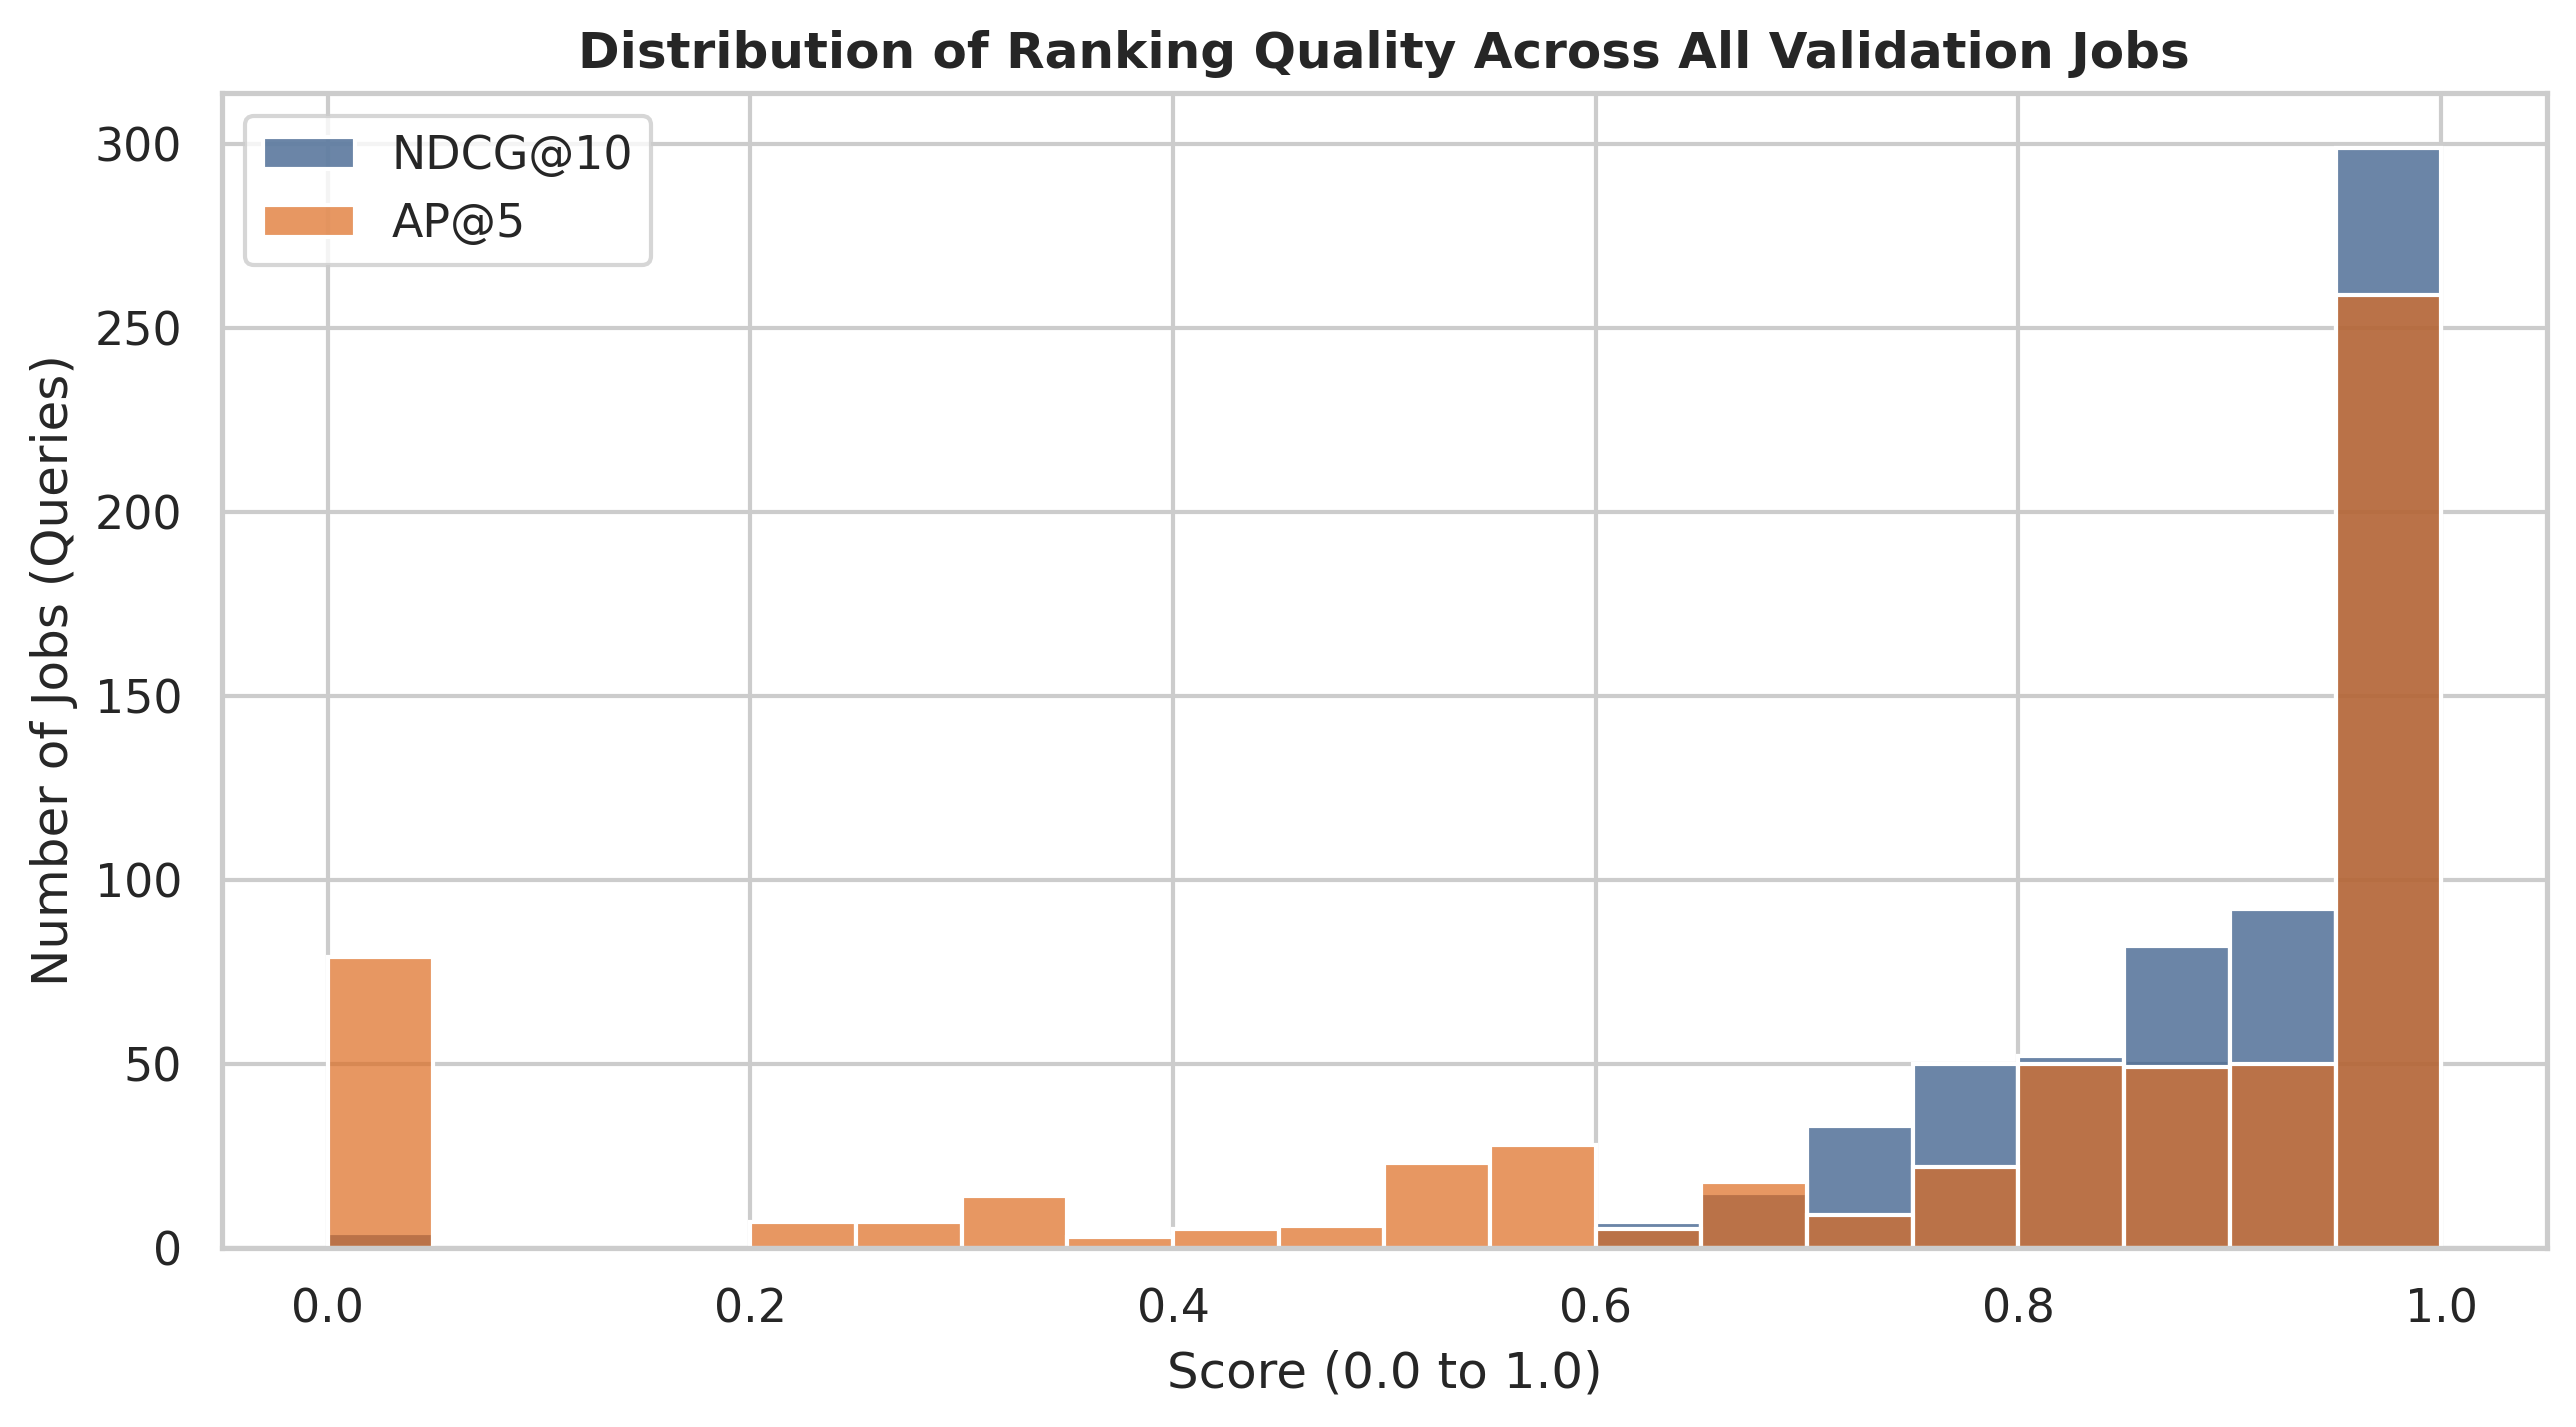
\includegraphics[width=0.9\textwidth]{06_evaluation_distribution.png}
    \caption{Distribution of NDCG@10 and AP@5 scores across all queries (jobs) in the temporal validation set.}
    \label{fig:evaluation_dist}
\end{figure}

\subsection{Final Inference \& Conclusion}
Applying the principle of Occam's Razor, we recognized that while highly complex multi-model ensembles can sometimes yield marginal gains, a robust, single well-tuned LightGBM Ranker is vastly superior for production-level stability. For the final submission, our champion model inferred unbounded continuous margins (log-odds) across the unseen test set. The final output was saved with strict adherence to the original test indices, ensuring the platform's backend could internally group and rank the scores accurately. 

The finalized pipeline successfully resolved the extreme data imbalance, resulting in a final evaluation score of \textbf{84}.

% ==========================================
% CONCLUSION
% ==========================================
\clearpage
\section{Conclusion}
This assignment highlighted the fundamental differences between standard tabular modeling and domain-specific challenges. From fraud detection constraints in early tasks to the complexities of Information Retrieval and LambdaRank in Task 3, our approaches emphasized robust feature engineering and strict data-leakage prevention. The successful implementation of techniques like Out-of-Fold Target Encoding and cross-table interaction metrics ultimately proved to be the defining factors in achieving high predictive performance across all tasks.

\end{document}